\chapter{Software Development in ROS2}\label{c:ros}

Robotic systems have emerged into several scenarios, where its usage ranges between basic processes automation, up to full performance over critical tasks, consequently causing the complexity increase in these domains. 

Due to the wide variety of robotic hardware presented in multiple domains, concerning about software development is rather difficult \cite{cousins2011exponential}. The reuse of code is non-trivial, and therefore, large-scale development is rendered untenable. The \textit{Robotic Operating System} (ROS) presents itself as a middleware system, created to facilitate robotic system development in large scale.

In ROS, software flexibility was prioritized above all else, meaning that values like security were disregarded. Thus, ROS-based applications tend to face increased security risks, related to the exposure of the whole robotic network. Due to the scale and scope of the robotics growth, security insurance must be addressed as a developing priority \cite{diluoffo2018robot, kim2018security}.

The upgraded version of ROS, \textit{Robot Operating System 2} (ROS2), presents itself as a framework for developing robotic systems, supported by the \textit{Data Distribution Service} (DDS) standard. Multiple middleware implementations are built over this standard, which provides numerous DDS-based specifications as well as valuable \textit{Quality of Service} (QoS) transport parameters.

The \textit{DDS-Security} specification \footnote{https://www.omg.org/spec/DDS-SECURITY/1.1/} aims to supply multiple plugins regarding the security domain. Consequently, ROS2 yields a wider command toolset compared to the former version of ROS, as they bring forth to a toolset, the \textit{Secure Robot Operating System 2} (SROS2) toolset, concerning the security functionality that DDS-Security plugins offer.

This chapter introduces necessary background information over the major concepts on which this thesis rests. First, it is presented a detailed introduction to the concepts around Robot Operating System (ROS), as well as the evolution approach that ROS faced towards providing security to its deployed systems. Regarding this goal, Data Distribution Service (DDS) and its integration on Robot Operating System 2 (ROS2) must be contextualized beforehand.


\section{Architecture Considerations}

The Robot Operating System was created by a collaborative open-source community, that has undergone rapid development \cite{cousins2011exponential} to contribute in the advancement of cyber physical systems. It was purposefully designed to be a development enhancer for the realm of robotic applications \cite{diluoffo2018robot, intro-ros}.

Fundamentally, ROS is a middleware, as it provides a custom serialization format, a custom transport protocol as well as a custom central discovery mechanism, presenting itself as a distributed layer between the top application layer and the operating system layer. 

ROS was designed to provide as much as modularity and composability to the application layer as possible \cite{casini2019response}, allowing ROS applications to be built over several software modules, as independent computing processes called \textit{nodes}. These compose together to fulfill the deployment characteristics of the corresponding robot \cite{maruyama2016exploring}.

\subsection{Former Architecture}

The Robot Operating System architecture is based on a hybrid peer-to-peer implementation, where network communication is done over message-passing through a publish-subscribe pattern. The communication API relied on a stateless XML-encoded remote procedure protocol. Transport libraries regarded the data exchange accounting serialization over sockets \cite{white2016sros, dieber2020penetration}.

The architecture emphasized on approaching communication through a centralization perspective. It relied on the explicit implementation of a \textit{Master node}, that controlled every aspect of the communication establishment. Consequently, every information exchange within the network had to go through this master.


\begin{figure}[H]
  \centering
  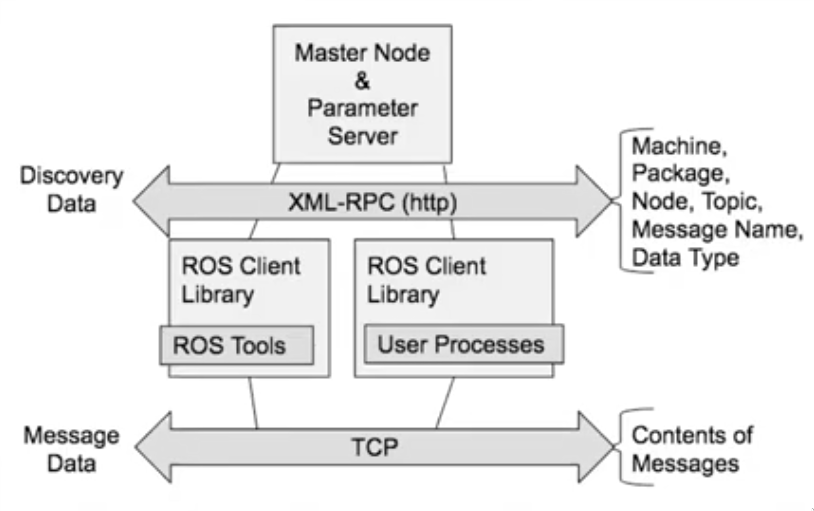
\includegraphics[width=0.6\linewidth]{img/former-ros1-architecture.png}
  \caption{Robot Operating System architecture.}
  \label{fig:ros1-architecture}
\end{figure}

Formerly, due to the sheer wide capabilities controlled by the master, this centralization approach was duly valorized. It naturally fits the purposes of a research tool, as it is simpler to monitor and analyze the system behaviour. However, because it is strongly reliant on the master node's availability, this communication architecture does not scale effectively, making it unsuitable for safety-critical or real-time applications. If the master fails, the entire system fails, representing a single point of failure and a huge performance bottleneck.

Many research communities tried to fix these real-time issues by proposing potential solutions, while supporting the same architecture design. Unfortunately, fell short of meeting the requirements of real-time applications. It became clear to the ROS community that the framework had architectural limitations that could not be rearranged using the same design approach \cite{maruyama2016exploring, dieber2020penetration}.

The Robot Operating System 2 comes as a complete refactoring of ROS, with the aim of increase the framework's real-time capabilities, by allowing the development of time-critical control over ROS, as it moves away from the former architectural design towards the implementation of an external middleware that can support the production needs of the outgrowing robotic systems \cite{kim2018security, casini2019response}.

\subsection{Data Distribution Service}

The Data Distributed System (DDS) \footnote{https://www.omg.org/omg-dds-portal/} is an \textit{Object Management Group} (OMG) middleware standard. The standard was developed to address the demand for enhanced interoperability across different vendors' middleware frameworks, directly addressing data communication between nodes that belong to a \textit{publish-subscribe} communication architecture, for real-time and embedded systems. 

A communication middleware aims to ease the complexity behind creating and maintaining communication architectures. It is responsible for handling relevant aspects like network configuration, communication establishment, data sharing and low-level details. As a result, system developers can mainly focus on their applications purposes, rather than concerning about information moving across levels \cite{dds-what-is}. 

DDS uses the \textit{Data-Centric Publish Subscribe} (DCPS) model as its communication model approach. DCPS is based on a publish-subscribe pattern, where the \textit{data-centric} messaging technique is implemented. It conceptually creates a virtual \textit{Global Data Space}, acessible by any DDS-based application, where data is properly delivered to the applications which quest for it, saving bandwith and processing power \cite{3, pardo2005introduction}. A \textit{domain participant} enables an application to participate in the Global Data Space, either as a \textit{publisher} or as a \textit{subscriber}, according to their role on data exchange \cite{maruyama2016exploring, alaerjan2017modeling, dcps-rtps}. 

\begin{figure}[H]
    \centering
    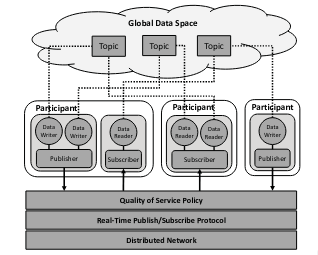
\includegraphics[width=0.4\linewidth]{img/dcps-model.png}
    \caption{DDS architecture: DCPS model with RTPS. Extracted from \cite{maruyama2016exploring}.}
    \label{fig:dcps-model}
\end{figure}

To properly address the data transportation through physical network, DDS offers a wire specification protocol called \textit{Real-Time Publish-Subscribe Wire Protocol} (RTPS) \cite{rtps}, providing automatic discovery between participants. This protocol also works under a publish-subscribe policy over best-effort transports, where data transmission between endpoints is handled \cite{yun2017data}. RTPS allows multiple applications, that could differ on their used DDS implementations, to interoperate with each other as network domain participants \cite{dcps-rtps, alaerjan2017modeling}.

Furthermore, RTPS was designed to employ Quality of Service (QoS) profiles, which allow for the specification of various transport policies, formerly not covered by DDS. This approach offers flexibility over communication configuration and development versatility, allowing the developer to specify whatever QoS satisfies its system's communication needs \cite{alaerjan2017modeling, diluoffo2018robot, maruyama2016exploring}. 

Briefly, DDS leverages the premise of a transport-independent virtualized \textit{Data Bus} to address network resources' distribution, in which stateful data is distributed through the network. The involved applications can access this data in motion, representing an architecture with no single point of failure, respectively enabling a realiable way of ensuring data integrity. Consequently, by adopting this approach, the load on the network is independent of the number of applications, making it easily scalable.

\begin{figure}[H]
    \centering
    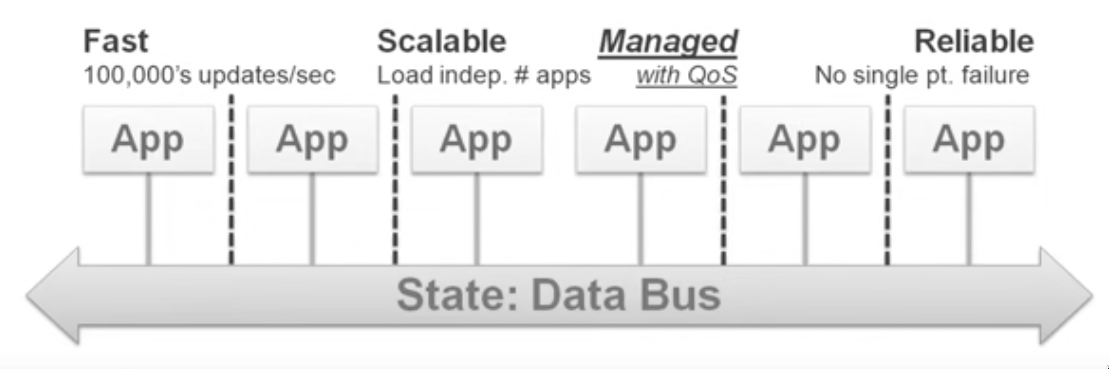
\includegraphics[width=0.6\linewidth]{img/dds-architecture.png}
    \caption{Data Distributed System architecture in a nutshell.}
    \label{fig:dds-architecture-nutshell}
\end{figure}


\subsection{ROS2-DDS Architecture}

As previously stated, the Robot Operating System 2 was developed to address the former architecture lack of support for real-time systems, mainly due to its architecture design that relied on their own middleware specification. To address this, ROS2 middleware approach is built upon the DDS framework \cite{maruyama2016exploring}, leveraging DDS for its messaging architecture, where communication and transport configuration are handled. 

As far as dependencies are concerned, DDS implementations have light sized dependencies, often related to language implementation libraries, easing the complexity behind installing and running dependencies \cite{ros-on-dds}.

The middleware's on-top layer regards the ROS client library (\textit{rcl}) \footnote{http://wiki.ros.org/Client\%20Libraries}, already implemented in the former ROS architecture. This layer accounts the availability of ROS concepts to the Application layer, as it provides APIs to ease the software implementation by ROS developers \cite{ros2documentation}. As ROS aims to support different programming languages over the same computing context, each language-specficic API must have its corresponding client library (\textit{rclcpp} regarding \textit{C++} and \textit{rclpy} regarding \textit{Python}). The \textit{rcl} accounts these client libraries by abstracting their specification, consequently reducing code duplication \cite{rcl, casini2019response}.

\begin{figure}[H]
    \centering
    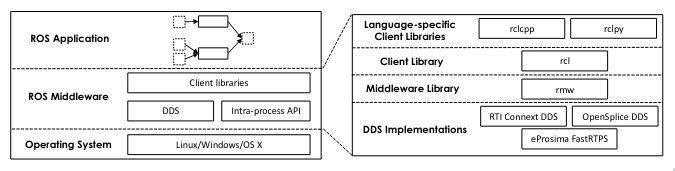
\includegraphics[width=\linewidth]{img/ros2-architecture.png}
    \caption{ROS2 framework architecture.}
    \label{fig:ros2-architecture}
\end{figure}

Towards supplying a wide range of configurations back to application layer, ROS2 aims to support multiple DDS implementations, in which these implementations API specification might differ from each other (currently, \textit{FastRTPS} by \textit{eProsima}, \textit{Connext} by \textit{RTI}, and \textit{Vortex OpenSplice} by \textit{Adlink}). It should be noted that the DDS implementations are low-level of abstraction, strictly defined by its corresponding vendor's API. DDS only defines fundamental procedures at a higher degree of abstraction.  

In order to abstract \textit{rcl} from the specifications complexity of these implementations APIs, an DDS-agnostic interface is being introduced, the \textit{rmw} (ROS MiddleWare) interface \cite{casini2019response}, allowing portability among DDS vendors, which consequently enables ROS developers to interpolate DDS implementations, based on their applications needs during runtime. The information flow through the middleware layer is done over structure mapping between ROS and DDS data models, addressed by the \textit{rmw}, regarding the DDS implementation that is being considered at runtime.

\subsection{Computation Graph}

From a logical perspective \cite{casini2019response}, ROS applications are composed of many software modules that operate as computation nodes, allowing its participation into the ROS Global Data Space. The use of publish-subscribe model approach as communication type, through message-passing patterns, confers additional concept complexity to the application architecture, where the latter can be naturally represented as a computation graph \cite{cousins2010welcome}.

The application's computation graph presents itself as a graphical network, where runtime named entities have their unique role when it comes to data distribution.

\subsubsection{Node Instances}

The application development is done over package orchestrating, where each logically represents a useful software module. Packages might be compromised by numerous \textit{nodes}, that can be perceived as processes that will likely perform computation over the network. It is worth mentioning that, nodes can be connected within a single package or between multiple packages, as they are built over their corresponding packages \cite{cousins2010welcome, intro-ros}.

Thus, the network is comprised by many nodes, running simultaneously and exchanging data between them, where each node addresses its corresponding network module purpose \cite{ros2documentation}. Fault tolerance features are guaranteed as nodes have their corresponding unique name, allowing communication in an unambiguous manner, which confers a suitable approach when developing a complex robotic system.

The notable usage of callback functions provide great functionality when it comes to manage node's behaviour in the communication process. Additionally, \textit{timers} can also be used, since they provide a useful way of managing these callbacks, by time-assigning.

\subsubsection{Communication}

Message-passing is the primary means by which nodes communicate with one another. The \textit{message} definition is a well-typed data structure, which commonly characterizes every data structure concerning the information exchange between nodes. A message is defined by its data type, also known as its \textit{interface}, which can either be primitive (\textit{integer}, \textit{string}, \textit{boolean}, among others), or defined by a complex data structure, where multiple data types are assigned to their corresponding variables \cite{ros2documentation, intro-ros}.

ROS computation graph provides \textit{3} different ways of establish node communication, those being \textit{Topics}, \textit{Actions} and \textit{Services}. These communication mechanisms have different interfaces, specified in different folders with unique namespaces \cite{ros2documentation}.

Topics are perhaps the most common method, naturally perceived as middle-communication buses, over which messages are passed through. As semantic approach, communication through topics is handled by the publishing-subscribing pattern. A node publishes the message to any number of topics, that are then subscribed by nodes that want to get access to that message. Topics provide a multicast routing scheme, where publish data is casted into the multiple nodes that are subscribed to the topic \cite{casini2019response}.

\begin{figure}[H]
    \centering
    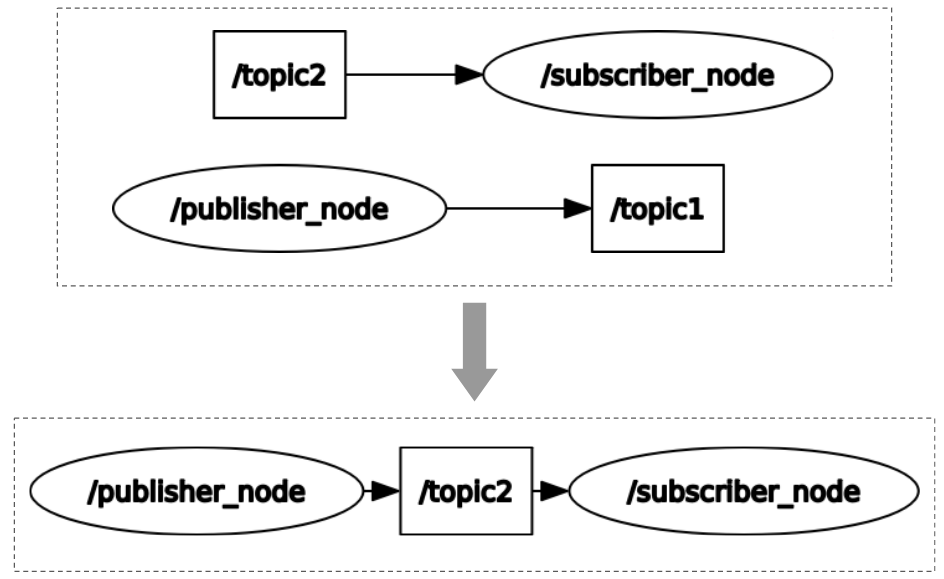
\includegraphics[width=0.5\linewidth]{img/ros2-topics.png}
    \caption{Communication behaviour over \textit{topics}.}
    \label{fig:ros2-topics}
\end{figure}

A specific \textit{topic} is created upon specifying its entity name over either a publisher or a subscriber callback instance. Whenever a node creates a publisher, intentionally instantiated to publish a message through a specified topic, \textit{roscore} is used to advertise the latter, enabling message passing to the corresponding topic subscribers. Message processing is done via the node's callback functions, which are activated upon message receipt, as it can also be utilized for publishing purposes \cite{casini2019response}.

Even though topics are the most conventional way of communication, due to its multicast scheme, subscribers can not be identified by the publishers, so logging and synchronization becomes rather difficult \cite{intro-ros}.

The use of services enables a client node, that can also be seen as a topic subscriber, to request data from a server, that likewise a topic publisher, furnish data through a service. This is a bidirectional synchronous form of communication based on a request-response pattern.

Other notable way of exchanging data is by setting goals through Actions. Actions are intended to process long-running tasks, where the client sends a goal request to the server node, that confirms the receiving of this goal. The server might provide feedback to the client before providing a response to the client. 


\subsubsection{Launch Files}

A conventional way of deploying a ROS application is through the use of launch files, enabling the multi-configuration over entire robotic applications, where network nodes can be individually pre-configurated. Therefore, ROS makes use of the \textit{roslaunch} to automatically initialize the whole network, simultaneously launching each node \cite{intro-ros}. This provides a simpler way of monitoring the system nodes. 

The Figure \ref{fig:ts-rqt-graph} depicts the network architecture corresponding to an ROS application well-known example called the \textit{TurtleSim}. This application is mainly composed by \textit{2} nodes, that perform together towards moving a turtle. Additional nodes were implemented, in order to add complexity to the current network, as to later support security as a proper example. Briefly, the \textit{multiplexer} node acts as a topic selector between two different subscribed topics, where each of them was respectively associated with a priority value. Based on the priority valued, the \textit{multiplexer} node forwards the commands, related to the selected topic, into the \textit{turtlesim} node, triggering the turtle's movement. 

The \textit{rqt} \footnote{ROS provides a GUI tool called \textit{rqt}, that assists developers in manipulating the network elements, in a more user-friendly manner.} visualizer, \textit{rqt\_graph}, allows the developer to perform analysis over a graphical visualization of the network computation graph.

\begin{figure}[H]
    \centering
    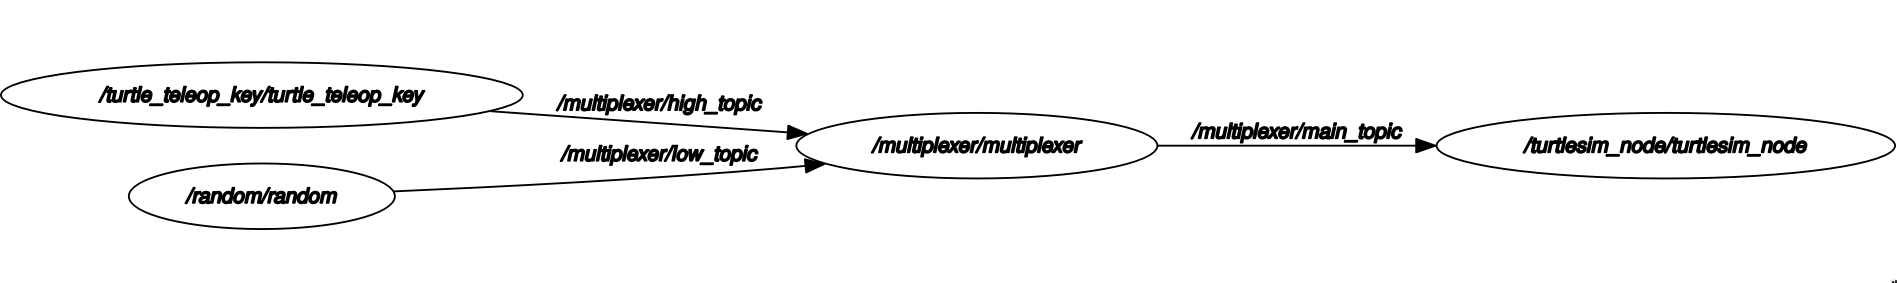
\includegraphics[width=0.8\linewidth]{img/ts_rqt_graph.png}
    \caption{\textit{TurtleSim}'s network graph presented by \textit{rqt\_graph}.}
    \label{fig:ts-rqt-graph}
\end{figure}

After the proper configuration of each node regarding the \textit{TurtleSim} example, the network can be easily managed and automatically launched through a launch file. The Figure \ref{fig:ros-lf} addresses the launch specification related to the latter application.

\begin{figure}[H]
\begin{lstlisting}[otherkeywords={launch, node, name, pkg, exec, output}]
<launch>
    <node name="turtlesim" pkg="default" exec="turtlesim" output="screen"/>
    <node name="keyboard" pkg="default" exec="keyboard"/>
    <node name="random" pkg="random" exec="random"/>
    <node name="multiplexer" pkg="multiplexer" exec="multiplexer"/>
</launch>
\end{lstlisting}
\caption{\textit{TurtleSim} launch file.}
\label{fig:ros-lf}
\end{figure}

Additional node configuration, such as name remapping and parameter adjustments, can be specified under the \textit{args} tag, which offers great functionality to the launching process. 

Distinctive namespaces allow the system to start the nodes, without any name nor topic name conflicts. However, this technique has some flaws attached, since it does not furnish a way of launching nodes in a separated terminal, often needed for user interaction purposes, like input reading.

\subsubsection{Parameters}   

Another relevant concept behind ROS is the existence of nodes parameters, that allows individual configuration of the network nodes. In the former version of ROS, the node parameters were controlled by a global \textit{Parameter Server}, managed by its corresponding ROS Master \cite{intro-ros}. However, in ROS2 each node declares and manages its own parameters, by using the predefined commands \textit{get} and \textit{set}. Additionally, using a parameter function callback, the node's parameters can easily be edited \cite{ros2documentation}.
        
\subsubsection{Node Composition}  

Usually a node is attached to a single process, but it is possible to combine multiple nodes into a single process, structurally abstracting some network parts, while improving the network's performance \cite{ros2documentation}. However, there is a slight difference about how ROS and ROS2 approaches node composition. 

In the former version of ROS, node composition was done over the combination of \textit{nodelets}, intentionally designed to ease the cost of overusing TCP for message-passing between nodes \cite{ros-nodelets}.  Supported by the former idea of nodelets, ROS2 introduces the \textit{components} as software code compiled into shared libraries, that can be loaded into a \textit{component container} process at runtime in the network, ensuring node composition \cite{ros2documentation}. 

%Node composition could also be applied for security matters. Suppose a scenario where multiple nodes respect the same security policies. By combining them into a single process, the mapping into this set of rules would be direct, easing the usage of security enclaves.
           

\section{Security}

The deployment of real-time systems implies critical concerning about safety and security \cite{maruyama2016exploring}, resulting of the demanding time-critical scenarios. 

Robotic systems fall under the umbrella of this broad system definition, as they feature unique cyber vulnerabilities related to its integration over highly networked environments, that confers great importance on exposing critical time-reliant scenarios \cite{mcclean2013preliminary, dieber2017security}.

\subsection{Former ROS Security Concerns}

The network security evaluation in a system is done by applying several analyzing techniques. Generally, these techniques do not cover every security aspect, as new vulnerabilities arise from technology evolution \cite{kaeo2004designing}.
The appliance of security countermeasures techniques upon configuring the system's network confers a critical step when aiming towards achieving security.

Within this vast topic, several avenues of endeavor come to mind, each deserving of a substantial study. Network security entails pre-exploration of the system's network through practical networking security techniques, such as intrusion detection and traffic analysis \cite{marin2005network}.

Numerous researchers \cite{8794451, dieber2020penetration} have investigated the use of these techniques, such as port scanning and penetration testing, over the previous version of ROS in order to thoroughly assess attack vulnerability throughout the ROS architecture. 

The ROS Master role in the communication architecture, and its ability to connect to other nodes, imposes many concerns about how to address security to ensure protection over the Master node. Exposing this node poses a critical threat over the whole network \cite{8794451}. 

Moreover, there were also worries regarding the way ROS handled node communication. Network security may be jeopardized, as a result of the publish-subscribe pattern transparency, where node-to-node communications are settled in plain text, making data content vulnerable to unauthorized usage \cite{kim2018security, white2016sros}. Additionally, the former API did not confer any message integrity technique, making applications vulnerable to packet sniffing and man-in-the-middle attacks \cite{white2016sros}.
 
However, due to the high non-linearity and complexity of real-time systems, implementing such thorough analysis method in near real-time remains a significant difficult task \cite{diao2009design}.

\subsection{DDS-Security Specification}

The Object Management Group accounts security integration by supplying an in-depth specification, consequently adding features to the already developed DDS standard. The DDS-Security is a specification that serves as a security extension to the DDS protocol, defined by a set of plugins (Authentication, Access Control, Cryptographic, Logging, Data Tagging), combined in a \textit{Service Plugin Interface (SPI)} architecture \cite{8442103, ros-dds-integration}.

\begin{figure}[H]
    \centering
    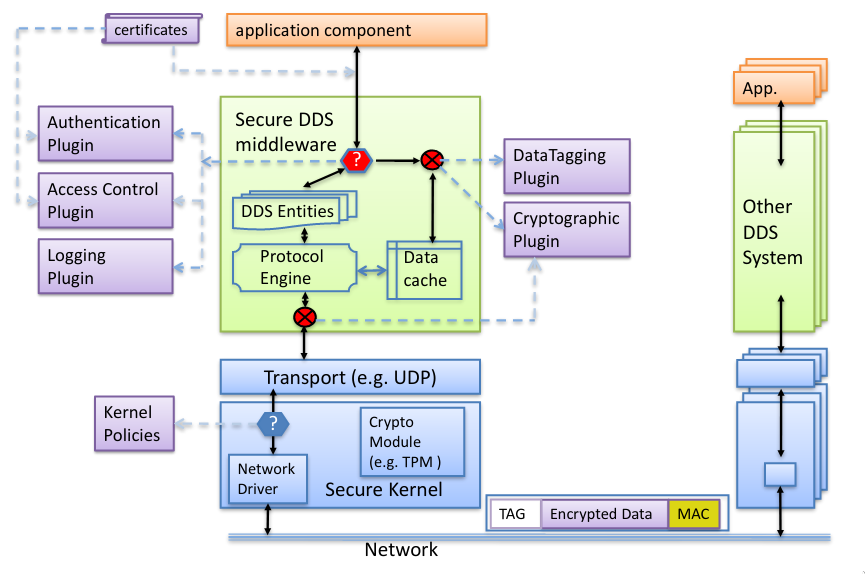
\includegraphics[width=0.7\linewidth]{img/dds-security-architecture.png}
    \caption{DDS-Security Architecture. Extracted from \cite{dds-s}.}
    \label{fig:dds-security-architecture}
\end{figure}

This specification enables its integration by furnishing a \textit{Security Model} supplied to the DDS standard, whereas the \textit{Service Plugin Interface} architecture is responsible for granting plugin enhancement for compliant DDS implementations. Moreover, depending on the security requirements needed for a particular application, these plugins might be adjusted by the latter's runtime DDS implementation \cite{dds-s}.

\subsubsection{Authentication}

Upon considering a secure environment over the DDS Global Data Space, data integrity can not be prone to unauthorized usage. Therefore, data exchange requires verification procedures to properly identity the authenticity each DDS domain participant.

The Authentication plugin confers the most valued plugin to the entire SPI architecture, as it provides means to validate the identity of the application, later regarded as a domain participant \cite{dds-s, ros-dds-integration}. 

Each participant must be authenticated prior to entering the data space \cite{white2019network}. Therefore, participants are presented to the secured environment regarding the \textit{Public Key Infrastructure} (PKI). This latter is in charge of issuing asymmetric keys to each participant, a \textit{public} and \textit{private} key respectively, that are used for both authentication and encryption procedures \cite{diluoffo2018robot, ros-dds-integration}. 

Moreover, regarding the issuer identity, the PKI provides an \textit{X.509 certificate}, that maps a distinguished domain name (DN) to the participant's public key \cite{diluoffo2018robot, white2016sros}. This certificate is accountable and signed by a trusted certificate authority (CA) \cite{white2019network, white2016sros, ros-dds-integration}. It ensures authenticity between asymmetric key pairs (both public and private) \cite{diluoffo2018robot}. 

The communication establishment over different participants must be preceded by a mutual handshake, where keys and certificates are exchanged to guarantee their authenticity \cite{white2019network, kim2018security}. Additionally, the DDS permissions of a domain peer are also concerned within this handshake. The control over permission distribution is respectively handled by the Access Control plugin.

\subsubsection{Access Control}

As aforementioned, the defined DDS specification handles policy control over the DDS domain through the Access Control plugin, where authenticated parties respective operations are imposed by policy restrictions \cite{dds-s, white2019network}. Domains within the Global Data Space are controlled over a set of DDS-related capabilities, that are either assigned or restricted to the authenticated participants \cite{ros-dds-integration}. 

Authenticated participants must be granted access to certain domains, where their roles on data transportation must be accordingly accounted by access permissions. If a participant is perceived as a domain data publisher, the domain restrictions must provide publishing privileges to its data topic \cite{white2019network}. 

Following the authentication procedure, domain authorization is also concerned using the proven PKI \cite{ros-dds-integration}, by embedding policy definitions through certificate extensions \cite{white2016sros}. 

Furthermore, the Access Control plugin employs \textit{2} configuration documents that are allocated to each participant \cite{white2019network}. This provides significant security capability, which is given as a supplement to the authentication procedure.

\textbullet\ Domain Governance: \textit{XML} document defining the domain's security policy.

\textbullet\ Participant Permissions: \textit{XML} document containing the permissions assigned to a given domain participant.

Notably, these configuration files are signed by a trusting Certificate Authority (CA) \cite{ros-dds-integration}. The CA's Permission Certificate confers protection against elevation of privilege attacks. Therefore, if the policy integrity is jeopardized, the handshake establishment between authenticated parties fails to commence \cite{white2016sros}.

\subsubsection{Communication and Encryption}

% The DDS-Security specification ensures encryption and authentication using \textit{OpenSSL}, while accounting security functions based on encryption standards \cite{takemoto2019performance}. Accordingly, it implements a handshake-based standard, concerning the \textit{OpenSSL} protocols, \textit{Secure Sockets Layer} (SSL) and \textit{Transport Layer Security} (TLS), which are used respectively used to ensure encryption over the network communication \cite{white2016sros, kim2018security}.

%The handshake is used to achieve mutual authentication within participants over the DDS domain. As stated, each participant must be authenticated prior to entering the data space \cite{white2019network}. Therefore, participants are presented to the secured environment regarding the Public Key Infrastructure (PKI). This latter is in charge of issuing a public certificate, accountable and signed by a trusted certificate authority (CA) \cite{white2019network, white2016sros}.

The DDS-Security specification ensures encryption and authentication using \textit{OpenSSL}, while accounting security functions based on encryption standards \cite{takemoto2019performance}. 

Accordingly, it implements a handshake-based standard, concerning the OpenSSL protocols, \textit{Secure Sockets Layer} (SSL) and \textit{Transport Layer Security} (TLS), which are used respectively used to ensure encryption over the network communication \cite{white2016sros, kim2018security}. The handshake is used to achieve mutual authentication within participants over the DDS domain \cite{white2019network}.

Following the participant key assignment, the \textit{Diffie-Hellman} key exchange protocol properly accounts the mentioned handshake, allowing both participants to exchange data over a shared secret key \cite{kim2018security}. % while accounting their own public certificate information \cite{kim2018security}. 
It enjoys the inter-exchange of both asymmetric keys, issued to each domain participant during the domain authentication procedure, in order to perform sign (using the private key) and verify (using the public key) operations \cite{kim2018security, diluoffo2018robot}.

The \textit{rcl} is capable of handling this DDS security requirement, levering ROS-based applications to support SROS2, accounting nodes as authenticated participants \cite{white2016sros}. 

As communication establishment is duly achieved throughout this handshake process, the DDS-Security specification takes advantage of the \textit{AES-GCM} encryption standard concerning data encryption over the implicit channel \cite{kim2018security, takemoto2019performance}.

\begin{figure}[H]
    \centering
    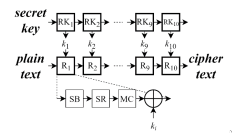
\includegraphics[width=0.4\linewidth]{img/ros_aes.png}
    \caption{\textit{Advanced Encryption Standard} algorithm. Extracted from \cite{takemoto2019performance}.}
    \label{fig:ros_aes}
\end{figure}

The key cryptosystem algorithm \cite{takemoto2019performance} presented in the \textit{Advanced Encryption Standard} (AES) considers the usage of functions towards achieving data encryption over the established communication. It enables configuration over data encryption, allowing both block and streaming transfer of ciphered data \cite{diluoffo2018robot}.

Here, the algorithm combines the shared key established with the message passed over the secure channel. Moreover, it is desirable to implement the \textit{Galois MAC (AES-GMAC)} encryption algorithm, that is based on block cipher operations, consequently adding encryption functionality to the AES algorithm, through a \textit{Message Authentication Code (MAC)} encryption function \cite{takemoto2019performance, kim2018security}.

Every cryptography-related operations are handled by the SPI's Cryptographic plugin. Naturally, these cryptographic capabilities, linked to the asymmetric key cryptography, are then used by both Authentication and Access Control plugins, ensuring authenticity support over their corresponding opearations \cite{ros-dds-integration, diluoffo2018robot}.

\subsection{Security Integration in ROS2}

As result of the DDS implementation as a flexible middleware interface in the ROS2 architecture, issues regarding security is no longer mainly ROS-dependent. Thus, when it comes to addressing security over communication, and subsequently data protection enhancement, ROS2 is heavily reliant on how the DDS standard is able to manage security \cite{kim2018security, 8794451}.

Every DDS implementation supported by ROS2 makes use of the DDS-Security specification, enabling security over ROS's application environment. Even though ROS2 is deployed without security mechanisms by default \cite{ros-dds-integration}, ROS2 provides a toolset, the Secure Robot Operating System 2 (SROS2) toolset \footnote{https://github.com/ros2/sros2}, extending ROS2's functionality to make use of the DDS-Security functionality. 

The control over these tools are done by \textit{rcl}, providing security over the Application layer, while DDS is capable of providing security over the communication architecture \cite{kim2018security}. SROS2 configuration is done over applying a set of security files to each ROS2 participant, with regard to how DDS handles certificate assignment to their participants \cite{white2016sros, ros-dds-integration}. 

Consequently, the toolset allows certificate generation and allocation through a keyserver directory, where security enclaves and their respective authentication files are stored inside subfolders \cite{white2016sros, ros-dds-integration}. Moreover, SROS2 enables the keyserver configuration in a flexible way, allowing developers to restricit certificate and CA attributes to an arbitrary number of nodes, defined over the same namespace \cite{white2016sros}.

The variety of capabilities in SROS2 toolset attempts to aid with security configuration across environments \cite{ros-dds-integration}. However, managing certificates and access control policies might lead to improper configuration. Additionally, orchestrating a real-time network towards achieving a secure environment confers to be a demanding process \cite{ros-dds-integration, white2019network}.

% The SROS2 configuration is done over applying a set of security files to each ROS2 participant, with regard to how DDS handles certificate assignment to their participants \cite{white2016sros}. The variety of capabilities in SROS2 toolset attempts to aid with security configuration across environments, however, the developer must be aware of improper configuration, that can still lead to security problems \cite{ros-dds-integration}.

\subsubsection{Security Enclaves}

As aforementioned, ROS2 relies on how handles DDS security over their \textit{Domain Participants}. DDS imposes the authentication of each participant prior to joining its Global Data Space, where the Certificate Authority and an established PKI comes in hand \cite{white2019network, white2016sros}.

Accordingly, the authentication process within the ROS2 network relies on the notion of a network enclave, where authentication and control artifacts are stored to properly achieve security over the network data space \cite{ros-security-enclaves}. Conceptually, an enclave is a secure region in the application address space that maintains confidentiality and integrity, while computations are being carried out on data.

Previously, a node was perceived as a separated DDS participant. However, by considering node composition as a reliable way of matching multiple nodes simultaneously to the same security domain, this node perception as participants can not be taken into account, due to causing non-negligible overhead, as memory space becomes rather difficult to handle \cite{ros-security-enclaves, ros-access-control}.

Concerning the enclave authentication procedure, its security artifacts must be addressable by a DDS participant, where the latter is associated to a node sharing context, instead of being perceived as a single node \cite{ros-security-enclaves}. Thus, when it comes to apply different policies over different nodes, that are matched in the same node context, a set of node profiles can be specified under the enclave notation. 
 
\vspace{0.5cm}
\textbf{Access Control within Enclaves}

The SROS2 toolset offers a well-typed markup language \textit{XML schema} \cite{ros-access-control}, where security policies bind profiles to access permissions for network objects, granting privileges back to a certain profile. \textit{Profiles} are implemented under the \textit{enclave} declaration, to duly support the node composition into a single process, enabling the possibility of combining multiple profiles, respectively addressing its corresponding node. % Typically, each \textit{enclave} declaration is linked to a corresponding ROS node, naturally perceived as a DDS participant.

\textit{Objects} are classified over a subsystem type, structurally characterized by permissions tags. Then object privileges are controlled over access values, either \textit{allow} or \textit{deny}, attributed to their corresponding permissions tags \cite{ros-access-control, white2018procedurally}. Briefly, each node profile is assigned to policies that concern some object identifier (OID). Each OID maps to a specific action, that is identified over an access value, allow or deny respectively \cite{white2016sros}.

The policy design approach works under the \textit{Mandatory Access Control}, that denies any privilege by default. The only way of allowing access to any object, is by explicitly specifying the subject's privilege access \cite{ros-access-control, white2018procedurally, white2016sros}. Naturally, this policy approach confers great value towards security, since it denies any attempt of privilege gaining attack by ROS-based packages from non-trusted sources \cite{white2016sros}.

Depicted in the Figure \ref{fig:ros-access-file}, it is presented a policy file where access control privileges are distributed across enclaves, and their inherited profiles. Recall the \textit{TurtleSim} example, the following \textit{XML} policy file addresses the access to topics for each respective enclave. 

\begin{figure}[H]
\begin{lstlisting}[otherkeywords = {xml, version, encoding, policy, version, enclave, enclaves, profile, profiles, topic, topics, xmlns:xi, path, ns, node, publish, subscribe, reply, request, call, execute, xi:include, href, xpointer}]
<?xml version="1.0" encoding="UTF-8"?>
<policy version="0.2.0" xmlns:xi="http://www.w3.org/2001/XInclude">
  <enclaves>
    <enclave path="/multiplexer">
      <profiles>
        <profile ns="/" node="multiplexer">
          <topics publish="ALLOW" >
            <topic>move_turtle</topic>
          </topics>
          <topics subscribe="ALLOW" >
            <topic>high_priority</topic>
            <topic>low_priority</topic>
          </topics>
        </profile>
      </profiles>
    </enclave>
    <enclave path="/turtlesim">
      <profiles>
        <profile ns="/" node="turtlesim">
          <topics subscribe="ALLOW" >
            <topic>move_turtle</topic>
          </topics>
        </profile>
      </profiles>
    </enclave>
    <enclave path="/keyboard">
      <profiles>
        <profile ns="/" node="keyboard">
          <topics publish="ALLOW" >
            <topic>high_priority</topic>
          </topics>
        </profile>
      </profiles>
    </enclave>
    <enclave path="/random">
      <profiles>
        <profile ns="/" node="random">
          <topics publish="ALLOW" >
            <topic>low_priority</topic>
          </topics>
        </profile>
      </profiles>
    </enclave>
  </enclaves>
</policy>
\end{lstlisting}
\caption{SROS2 policy file regarding the access control policies over the \textit{TurtleSim} example.}
\label{fig:ros-access-file}
\end{figure}

\section{Related Work}\label{s:relWork-sec}

The present section confers a notable overview over ROS security environment, that will focus on the following topics: It is intended to begin by presenting some works that demonstrate the absence of security over the ROS environment, that is then followed by some attempts regarding solutions; At last, ROS2-based studies will be given to contextualize the dissertation's main topic of study. 

Robotic systems were initially conceived as augmented computers with no explicit boundaries or limitations. As a result of the requirement to provide practical systems as fast as possible, security matters were disregard \cite{white2018procedurally}. Network security entails cautious analysis of the system's network using realistic networking security procedures \cite{marin2005network}. Concerning the Robot Operating System and its role as a robotic application enhancer, numerous researchers have examined the usage of such procedures to perform a thorough analysis over the latter's architecture.

\citeauthor*{8794451} present a practical overview over ROS security, in which the \textit{IPv4 address space of the Internet} is explored with the goal of identifying vulnerable hosts. Port scanning was used as technique to expose mostly master nodes as they provide valuable information about their associated topics and node's parameters. The performed scans furnished information about hosts that could either be a sensor, an actuator or even a simulator. This study is rather relevant because of how easily can attackers gather information about potential robots, and control them further on, through the public Internet, making it unavoidable to develop mechanisms concerning security. 

Moreover, in \citenum{dieber2020penetration}, it is presented different pentesting tools that entails exploiting techniques over ROS-based systems, in order to provide a proper overview of possible security flaws. Foremost, \citeauthor{dieber2020penetration} present a \textit{.net-based pentesting} tool called \textit{ROSPenTo}, developed with the intention of investigating strategies for manipulating running ROS applications. The latter provides several command line techniques to jeopardize robotic networks, including the ROS parameter server, that confers great value to the running nodes. 

The other tool is called \textit{ROSchaos} wittingly designed for exploiting the Master API. It differs from the former tool, since \textit{ROSPenTo} mainly focused on exploiting ROS \textit{Slave API}, which covers the node-to-node communication and the receipt of messages from the Master, without directly addressing the ROS Master as a compelling target. Regardless matter how subtle such attacks are, exploiting the Master directly may still be appealing to attackers. 

These techniques confer great value to the domain of security exploration over ROS, where the \textit{XML-RPC} embedded API is divided and subsequently exploited according to the participants roles within the network. Besides raising awareness of the importance of security in ROS, it promotes developers to conduct penetration testing on their applications.

Following the challenges that arose as a result of executing exploitation techniques on the ROS framework, numerous solutions were proposed in response to the need to offer security assurance for robotic applications. 

One of the earliest research on the security improvement of the ROS framework was proposed by \citeauthor{mcclean2013preliminary} in \citenum{mcclean2013preliminary}. Here, the first take is to exploit and reason about unique vulnerabilities related to the nature of cyber-physical systems, where it is demanding to collect data for further consideration. Afterwards, it is presented a novel research tool to aid in cyber-physical security research, named as \textit{honeypot}, where it is desirable to monitor unauthorized attempts to jeopardize these systems. Due to the significant information offered, the latter gives a basic yet crucial study on ROS, which acts as assistance to steer the development of future work in the burgeoning subject of cyber-physical security. 

% Another worth-mentioned research is presented in \citenum{crick2017rosbridge}. The latter describes the \textit{rosbridge} middleware that adds to the former ROS architecture an abstraction layer. It provides a socket-based interface through a technology standard, where minimalist services are accessible to developers.

In \citenum{white2016sros}, \citeauthor{white2016sros} addresses the security deployment over ROS in a more concise way, by proposing the \textit{Secure Robot Operating System} (SROS) as a planned enhancement to the former API, that includes mechanisms such as authentication, access control and cryptography measures. SROS seeks to provide adequate security architecture while minimizing existing user disturbances such as computational cost and API breaking. The final remarks regard the alternative usage of SROS, allowing developers to customize it to their own internal certificate formats. Moreover, \citeauthor{white2016sros} expects security logging and access control to evolve through well-defined standards, enabling more robust auditing and policy generating tools. 

Additionally, in \citenum{application-security-ros} it is presented a fairly pertinent research that recommends security improvements on the application-layer. Briefly speaking, the approach primarily focused on applying security measures on the application layer, by mainly running an Authentication Server, storing certificates and files related to trusted domain participants, while controlling and providing session keys related to the communication process. Topic-specific encryption keys are employed to protect data secrecy. However, the discussed architecture is based on the assumption that issuing authentication certificates are manually handled. Despite encryption and authentication mechanisms, attacks regarding the exposure of the network, such as denial of service attacks, still persist which cannot be handled on the application level alone. 

\citeauthor*{breiling2017secure} continue to follow the previous work in \citenum{breiling2017secure}, through a hardened ROS core with transparent authentication, authorization, and encryption functionalities that do not require the manual specification of nodes. Furthermore, secure workflows and initial penetration testing are supported in \citenum{dieber2017security}, in which \citeauthor{dieber2017security} show an insight of security weaknesses in the ROS architecture design, with additional attempts that regard potential solutions to those problems.

Regarding the SROS \cite{white2016sros} initial proposal, White continued to provide security overview over the framework through subsequent studies \cite{white2018procedurally, white2019network}. In \citenum{caiazza2019enhancing}, \citeauthor*{caiazza2019enhancing} present several solutions regarding the lack of security measures that autonomous devices, often related to the robotics world, tend to face. The effort then moves on to evaluate the ROS framework in order to provide a high-quality understanding solution. It follows a pipeline of security measurements, where logging, access control and authentication certificates are discussed over several proposals. It provides a clear analysis over the security state-of-art of ROS, and the analysis clearly states that the lack of techniques to prevent communication threats imposes the most valued consideration over robotic networks. \citeauthor*{caiazza2019enhancing} conclude their work by stating some future improvements to their current solution. 

In \citenum{white2018procedurally}, \citeauthor*{white2018procedurally} address robotics security through a proposed framework that focuses on handling access control policies for robotic software, with the intention of adding functionality to SROS \cite{white2016sros}. The latter offers an interesting perspective on leveraging access-control through a well-typed markup language schema, the \textit{ComArmor} configuration language, where privileges of objects is explicitly defined over policies. Then, profiles are used to arrange these policies in a hierarchical manner, binding namespaces to objects privileges, utilizing attachment expressions with predefined permissions denoted as rules. Rules are defined as a set of permissions for a given object, where each permission has a corresponding value that could either be allow or deny. 

The evaluation of this policy schema as a proof of concept was done by implementing it in a cryptographic framework called \textit{Keymint}. The latter follows similar authentication and cryptographic patterns as the initial SROS \cite{white2016sros}, where security artifacts and document keys are stored in respective keystores. The incorporation of the ComArmor language into Keymint adds significant value to the framework since it allows for reasoning about how to manage policy control prior to implementing any authentication mechanism, such as generating permission and governance files. The framework is then tested using a standard ROS example of a basic publisher and simple subscriber interacting over a topic. Thus, this approach provides a methodical testing procedure where both application satisfiability and access control policies implementation are overviewed, adding significant value back to the framework as it is possible to define higher level policies to allow for transport-independent access control definitions.

The ComArmor configuration language, presented above in \citenum{white2018procedurally}, confers a great alternative to the SROS2 default policy schema. During the framework's evaluation process, \citeauthor{white2018procedurally} presents a set of gratuitous permissions within SROS2 template through a simple comparative study between both configuration languages. Thus, it discusses possible SROS2 vulnerabilities discovered during the development and experimentation the Keymint framework, emphasizing the importance of continuous security evaluation throughout design development cycle.

Following the deployment of DDS in Robot Operating System 2, the majority of security problems were alleviated. As a result, the literature on the network security enhancements provided by ROS2 is largely concerned with providing an overview of the trade-off between performance and security. Furthermore, various inquiry studies evaluate ROS2 performance in terms of response time and safety important circumstances \cite{maruyama2016exploring, casini2019response}, in which DDS capabilities are highly emphasized to properly evaluate ROS2.

A notable work is presented in \citenum{kim2018security}, where the security definition of DDS was explored using current security standards. Also, the implementation of the DDS protocol was evaluated using techniques of static analysis. It provides a framework for doing benchmark evaluations in various network and security configurations to reflect on the needs of real-time applications. Different performance time-related metrics and benchmark network scenarios (wired and wireless) were thoroughly investigated to give a well-based analysis over efficiency. The findings clearly illustrate that employing a reliable VPN application is more time efficient; nevertheless, SROS offers far more decentralized features than a VPN, which is typically desirable when designing a distributed system. \citeauthor*{kim2018security} conclude their work by reasoning about the security capabilities that DDS has to offer, after which a static code analysis of the DDS security implementation was undertaken. The research revealed that the latter did not conform to the security specfication by OMG. 

A pertinent research that examines the trade-off between performance and security is regarded in \textit{Robot Operating System 2: The need for a holistic security approach to robotic architectures} \cite{diluoffo2018robot}. Here, \citeauthor{diluoffo2018robot} conduct a thorough examination of Robot Operating System 2 and outlines possible hazards for this new robotic system paradigm. Thus, the DDS security specification is thoroughly examined in terms of performance versus security models and how security is integrated with ROS 2, as well as how the addition of security affects system design. 

As a result, \citeauthor{diluoffo2018robot} go on to present a systematic study of ROS2 in order to provide a good knowledge of how the system is built, and to subsequently undertake vulnerability analysis across various layers that require varying levels of protection. Additionally, the authors applied different performance metrics to duly present a well-based comparasion in whether security should be considered or not. Here, they consider the usage of DDS-based implementations, while addressing the RTPS communication protocol and it handles the communication and its configuration. The experiment illustrates that implementing security measures on protected data in motion results in a significant performance loss. 

Notably, they conclude with some recommendations towards security areas not duly covered by the DDS specfication, such as attacks stemming from
spy processes. They highlighted the preservation of the cognitive layer because of its importance in the robot itself, since all types of sensors that involve data collecting are concerned in that layer. Here, an advanced set of threats were described using Machine Learning, in which DDS is not capable of cover.

These presented works denote important considerations about how important is to address security over robotics, due to the variaty of attacks that might compromise their integrity. They follow the path of addressing vulnerabilities through applying security methods based on tools and protocols. However, studies regarding the appliance of quality analysis over static and property verification in ROS are quite limited. Despite this, the section \ref{s:relWork-pv} contains several works that advocate utilizing quality analysis to assess robotic systems.